\section{Програмна реалізація}
Особливості і деталі програмної реалізації

\subsection{Збір та попередня обробка даних}
Для збору даних та формування початкового датасету було створено допоміжний додаток у вигляді веб-ресурсу. Він являє собою веб-сайт, на якому здійснюються опитування серед різних класів респондентів: студентів, випускників та викладачів. Кожен учасник опитування заповнює невелику тематичну анкету, на основі якої формуюється таблиця вхідних даних. Загальну архітектуру додатку можна побачити на рис. \ref{fig:poll_architecture} 

\begin{figure}[h!]
  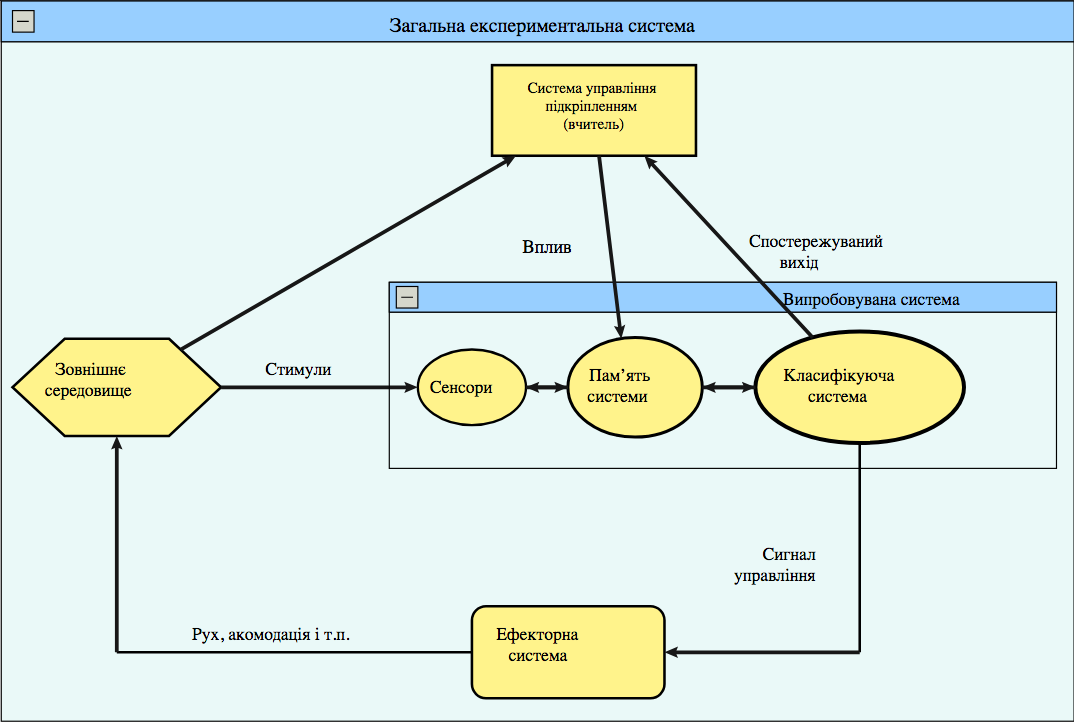
\includegraphics[width=\linewidth]{figures/fig_system.png}
  \caption{Загальна архітектура додатку опитування}
  \label{fig:poll_architecture}
\end{figure}

Особливості даних можна встановити ще на етапі їх збору. Навіть не здійснюючи жодного аналізу чи попередньої обробки можливо отримати деякі важливі характеристики даних або просто візуалізувати їх для зручнішого сприйняття чи для кращого усвідомлення того, з якого роду даними доведеться працювати. Саме для таких цілей і використовується \textit{exploratory data analysis} - аналіз даних з метою попереднього дослідження вхідних даних.

Візуалізація даних загалом здійснюється для таких цілей:
\begin{itemize}  
	\item Комунікативна складова:
	\begin{itemize}
		\item представити дані та ідеї;
		\item проінформувати;
		\item підтримати і аргументувати;
		\item вплинути і переконати;
	\end{itemize}
	\item Дослідницька:
	\begin{itemize}
		\item вивчити (дослідити) дані;
		\item проаналізувати ситуацію;
		\item визначити наступні кроки;
		\item прийняти рішення стосовно деякого питання;
	\end{itemize}
\end{itemize}

Оскільки одним із компонентів збору даних був \text{Google Spreadsheets}, то початкова візуалізація даних не становила жодної складності, тому що даний ресурс містить вбудовані засоби для цього рис. \ref{fig:answer_visualize} 

\begin{figure}[h!]
  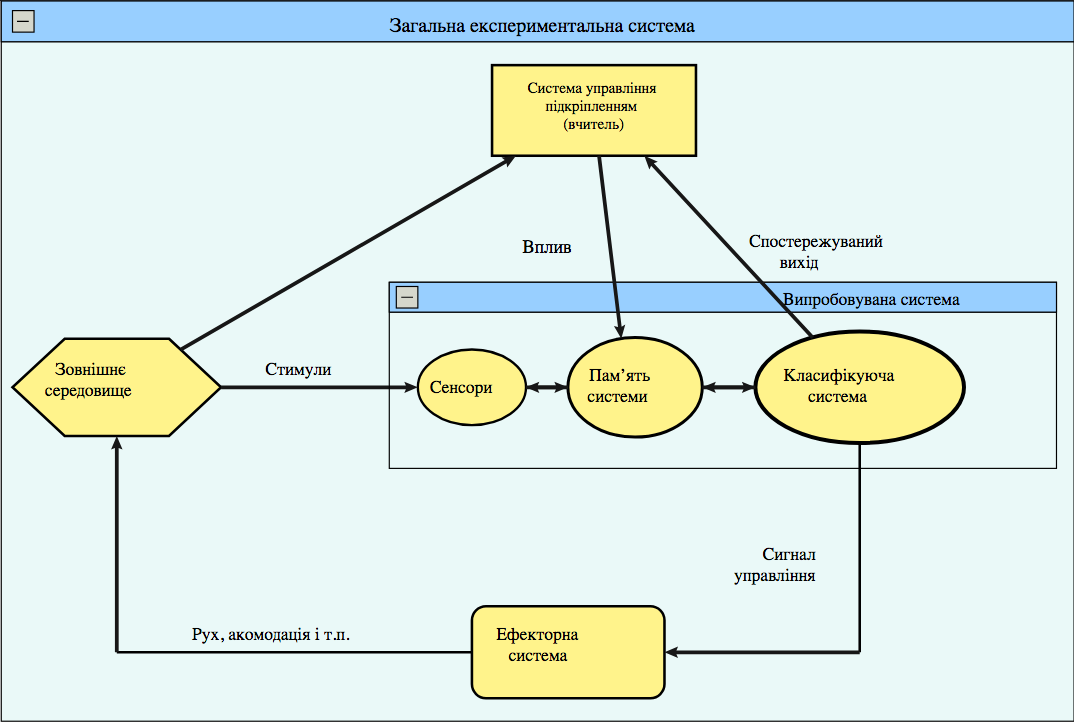
\includegraphics[width=\linewidth]{figures/fig_system.png}
  \caption{Візуалізація відповідей однієї з форм анкети опитування}
  \label{fig:answer_visualize}
\end{figure}

Для створення ефективної кінцевої моделі розроблюваний алгоритм повинен підповідати таким вимогам:
\begin{itemize}  
	\item відкритий доступ користувача до коду моделі на будь-якій платформонезалежній мові, що дозволить запускати її в довільному середовищі та не опиратися на використання сторонніх бібліотек;
	\item будова моделі та деталі її внутрішньої реалізації повинні бути відкритими, тобто користувач повинен мати змогу переглянути вихідний код і в разі необхідності самостійно відтворити довільний крок та отримати аналогічний результат передбачення для однакового набору вхідних даних;
	\item модель повинна мати точність максимально наближену до точності моделей, що показують найкращі результати для вибраних вхідних даних. Модель повинна мати аналогічні показники щонайменше для 95\% всіх вхідних наборів даних;
	\item виконання коду програми повинно бути швидким (близько 1 мс на рядок вхідних даних).
\end{itemize}